\section*{Appendix A\\Compactified Dimensional Architecture in\\Recursive Cosmology}
\addcontentsline{toc}{section}{Appendix A: Compactified Dimensional Architecture in Recursive Cosmology}
\label{appendix:A}

\subsection*{A.1 Dimensional Framework}

We posit that the recursive cosmology framework emerges from an M-theoretic bulk with eleven fundamental dimensions~\cite{witten1995string, becker2007string}, extended by one emergent informational degree of freedom. This yields a twelve-dimensional configuration structure:

\begin{itemize}
  \item \textbf{4 macroscopic spacetime dimensions:} \( (t, x, y, z) \),
  \item \textbf{6 compactified Calabi–Yau dimensions:} encoded in topological moduli (complex structure and Kähler parameters)~\cite{candelas1985vacuum},
  \item \textbf{1 emergent informational dimension} \( \mathcal{I} \): representing coherence memory and entanglement flux,
  \item \textbf{1 holographic boundary dimension:} supporting inter-cycle projection and entropy encoding~\cite{ryu2006holographic}.
\end{itemize}

\begin{figure}[H]
\centering
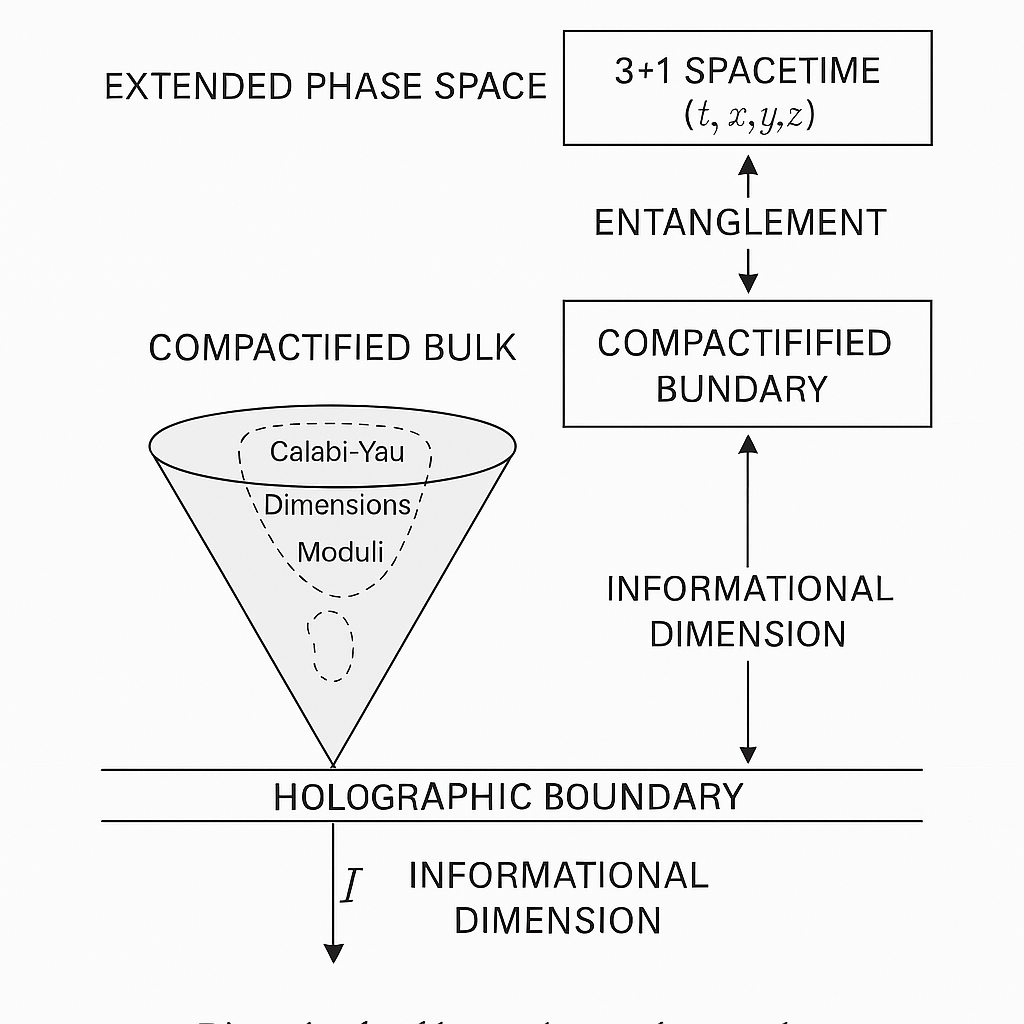
\includegraphics[width=0.75\textwidth]{figures/12D_structure_diagram.png}
\caption{Schematic of the proposed 12-dimensional recursive configuration space.}
\label{fig:12D_structure}
\end{figure}

\subsection*{A.2 Boundary Geometry}

Each cosmological cycle terminates on a boundary \( \Sigma_n \), defined by quantum extremal surface (QES) conditions~\cite{engelhardt2015coarse}:
\[
\Sigma_n = \arg\min_{\partial \mathcal{M}} \left( \frac{\mathrm{Area}[\partial \mathcal{M}]}{4G_N} + S_{\text{bulk}} \right)
\]
Here, \( S_{\text{bulk}} \) is the von Neumann entropy of the entanglement wedge. Partial data from \( \Sigma_{n-1} \) is projected holographically onto \( \Sigma_n \), enabling memory transfer across bounces~\cite{almheiri2019entropy}.

\subsection*{A.3 String-Theoretic Justification}

Within this embedding, inter-cycle information flow is mediated by Planck-scale excitations along wrapped M2- and M5-branes in the compactified dimensions. The Einstein–Rosen bridge (ERB) throat corresponds to a minimal-area hypersurface supported by non-trivial topology and vanishing brane tension~\cite{maldacena2013cool}:
\[
S_{\text{ERB}} \sim \frac{A_{\text{min}}}{4G_N} + i \lambda_E I(\phi, \phi')
\]
This structure generates the phase term \( \exp[i S_{\text{ERB}}] \) appearing in the recursion kernel \( K(\phi, \phi') \) (see Appendix~\ref{appendix:C2}), and encodes holographic entropy transport via entangled brane junctions.

\subsection*{A.4 Observational Consequences of Compact Geometry}

The Calabi–Yau moduli imprint oscillatory structure in the gravitational wave spectrum due to coupling between compactification scales and bounce dynamics. Frequencies \( f_j \) correspond to harmonics of the moduli length scale \( L_c \)~\cite{dienes1997string}:
\[
f_j \sim \frac{j}{L_c}, \quad j \in \mathbb{Z}^+
\]
These modulations yield harmonic dips or resonances in the gravitational wave background \( \Omega_{\text{GW}}(f) \), distinguishable from power-law features of inflationary models. Detection feasibility aligns with projected sensitivity of LISA, BBO, and DECIGO.

\subsection*{A.5 Summary}

This dimensional extension situates the recursive memory kernel and entanglement dynamics within a consistent M-theoretic and holographic framework. The 12-dimensional configuration space enables a structural origin for decoherence filtering and ERB-mediated entropy transport. The informational dimension \( \mathcal{I} \) is not spatial or metaphysical—it encodes coherence persistence across cycles.

Future work may explore topological transitions in the compact dimensions as potential triggers for decoherence resets, and investigate whether moduli instabilities act as stochastic drivers of recursive memory branching.
